\documentclass[11pt,a4paper]{article}

\usepackage[spanish,es-noshorthands]{babel}
\usepackage[T1]{fontenc}
\usepackage[utf8]{inputenc}
\usepackage{lmodern}
\usepackage[a4paper,margin=2.35cm]{geometry}
\usepackage{graphicx}
\usepackage{booktabs}
\usepackage{tabularx}
\usepackage{array}
\usepackage{amsmath}
\usepackage{hyperref}
\usepackage{xurl}
\usepackage{xcolor}
\usepackage{float}
\usepackage{caption}
\usepackage{enumitem}

\hypersetup{
    colorlinks=true,
    linkcolor=blue!60!black,
    urlcolor=blue!60!black,
    citecolor=blue!60!black
}

\setlength{\emergencystretch}{2em}

\title{Fase Residual sobre \texttt{Agent7250}:\\ motivacion, implementacion, barridos de alpha\_res y cierre metodologico}
\author{Proyecto EMG Prosthesis TD3}
\date{26 de marzo de 2026}

\begin{document}
\maketitle

\section{Objetivo y continuidad de la linea}

Este documento deja cerrada, de forma detallada, la fase de \emph{Residual TD3} construida como continuacion directa del benchmark operativo del proyecto: \texttt{Agent7250}. Si en notas previas aparece la referencia informal a ``Agent7200'', el checkpoint correcto y congelado como base del trabajo es \texttt{Agent7250}.

La idea central de esta fase fue no volver a entrenar una politica completamente nueva ni volver a modificar reward, observacion o cuantizacion. Se busco una intervencion mas conservadora: partir de una politica ya buena y aprender solo una correccion pequena sobre ella. Esa decision fue coherente con la lectura acumulada del repo:

\begin{itemize}[leftmargin=1.6em]
\item \texttt{Agent7250} ya hacia buen tracking.
\item Las ramas previas con regularizacion o warm-start tendian a politicas demasiado timidas.
\item El piloto de accion alineada al actuador tendio al extremo opuesto: mas borde y mas saturacion.
\item Hacia falta una forma de mejorar el compromiso tracking-esfuerzo sin destruir el prior ya aprendido por la politica base.
\end{itemize}

En la literatura, ese escenario encaja bien con \emph{Residual Policy Learning}: mantener un controlador base y aprender una correccion pequena y dependiente del estado, en vez de reemplazar la politica completa \cite{silver2018residual,schaff2020shared,resfit2025}. Esa fue la justificacion conceptual de esta fase.

\section{Punto de partida: benchmark congelado}

La fase residual se construyo sobre el mismo baseline valido que ya venia usando el proyecto desde la corrida correcta post-fix del simulador. Se mantuvo sin cambios:

\begin{itemize}[leftmargin=1.6em]
\item observacion \texttt{markov52},
\item reward \texttt{trackingMseActionRateReward},
\item TD3 feedforward,
\item remapeo y cuantizacion efectivos del actuador,
\item entorno corregido y ya validado tras el bug del simulador.
\end{itemize}

\begin{table}[H]
\centering
\caption{Benchmark congelado usado como referencia durante toda la fase residual}
\begin{tabular}{lr}
\toprule
Metrica & Valor \\
\midrule
\texttt{trackingMSE} & 0.043045 \\
\texttt{trackingMAE} & 0.160336 \\
\texttt{actionL2} & 0.596444 \\
\texttt{saturationFraction} & 0.392086 \\
\texttt{deltaActionL2} & 0.321385 \\
\texttt{absPWM mean} & 178.288566 \\
\bottomrule
\end{tabular}
\end{table}

Ese benchmark proviene de la linea de trabajo iniciada sobre TD3 continuo para protesis mioelectrica \cite{fuertes2026continuous}, en un contexto donde el control mioelectrico exige buen tracking pero tambien suavidad y estabilidad de accion \cite{chen2023review}. La arquitectura base sigue siendo TD3, adecuada para accion continua y ya implementada de forma nativa en MATLAB Reinforcement Learning Toolbox \cite{fujimoto2018td3,mathworks_td3_agent,mathworks_td3_options}.

\section{Por que la fase residual era una idea razonable}

La decision no fue arbitraria. Se apoyo en tres observaciones tecnicas del propio repositorio:

\begin{enumerate}[leftmargin=1.6em]
\item El benchmark ya estaba en una region util del espacio de politicas. No habia evidencia de que ``empezar otra vez'' fuera mejor que refinar una solucion buena.
\item Las intervenciones previas fallaban por exceso o por defecto: demasiado conservadoras o demasiado agresivas.
\item El problema ya no era aprender el movimiento base, sino corregir un compromiso fino entre tracking y agresividad.
\end{enumerate}

Residual Policy Learning fue propuesto precisamente para estos escenarios: cuando existe un controlador o politica base razonable, y conviene aprender solo el termino faltante \cite{silver2018residual}. Trabajos posteriores en control continuo y autonomia compartida refuerzan la misma idea: una correccion pequena y estructurada puede ser mas estable y mas eficiente que reemplazar toda la politica \cite{schaff2020shared}. En la misma direccion, lineas recientes de \emph{fine-tuning} residual sobre politicas preentrenadas vuelven a destacar que la forma mas segura de mejorar una politica fuerte es mantener la base y aprender un residuo con magnitud controlada \cite{resfit2025}.

\section{Que se implemento en el codigo}

La fase residual no fue un cambio difuso; se codifico como una rama experimental clara y trazable dentro del proyecto.

\begin{table}[H]
\centering
\caption{Archivos clave de la fase residual y su funcion}
\small
\begin{tabularx}{\linewidth}{>{\ttfamily\raggedright\arraybackslash}p{0.42\linewidth} >{\raggedright\arraybackslash}X}
\toprule
Archivo & Funcion \\
\midrule
\path{matlab_code/agents/agentTd3Residual7250.m} & Construye el nuevo agente residual a partir del checkpoint base \texttt{Agent7250}. \\
\path{matlab_code/agents/load_agent.m} & Incorpora el caso \texttt{td3\_residual7250} al flujo normal de carga. \\
\path{matlab_code/src/loadSavedAgent.m} & Estandariza la carga del checkpoint base y de checkpoints residuales. \\
\path{matlab_code/src/run_agent7250_residual_policy_pilot.m} & Lanza el piloto principal con \(\alpha=0.20\). \\
\path{matlab_code/src/run_agent7250_residual_continuation.m} & Continua desde el mejor checkpoint residual para evaluar si mas episodios ayudan. \\
\path{matlab_code/src/run_agent7250_residual_alpha_sweep.m} & Ejecuta el barrido corto inicial \(\alpha \in \{0.10,0.20,0.30\}\). \\
\path{matlab_code/src/run_agent7250_residual_alpha_refinement_sweep.m} & Ejecuta el refinamiento fino \(\alpha \in \{0.18,0.20,0.22,0.25\}\). \\
\path{matlab_code/src/reconstructResidualPolicyDiagnostics.m} & Reconstruye en postproceso la descomposicion entre accion base y correccion residual. \\
\path{matlab_code/src/@Env/step.m} y \path{saveEpisode.m} & Guardan estado, accion final y logs necesarios para diagnostico residual. \\
\path{matlab_code/src/summarizeEpisodeDirectory.m} & Agrega las metricas residuales por episodio y por corrida. \\
\bottomrule
\end{tabularx}
\end{table}

La implementacion se apoyo en componentes ya disponibles en MATLAB para TD3 y actores deterministas continuos basados en \texttt{dlnetwork}, asi como en capas funcionales para componer ramas dentro del actor \cite{mathworks_continuous_actor,mathworks_function_layer}.

\section{Que es exactamente alpha\_res}

La politica residual se definio como una composicion entre:

\begin{itemize}[leftmargin=1.6em]
\item una politica base congelada, \(a_{\mathrm{base}}(s)\), tomada de \texttt{Agent7250},
\item y una correccion aprendible, \(a_{\mathrm{res}}(s,a_{\mathrm{base}})\).
\end{itemize}

La accion final se construyo como:

\[
a(s) = \mathrm{clip}\Big(a_{\mathrm{base}}(s) + \alpha_{\mathrm{res}}\, a_{\mathrm{res}}(s,a_{\mathrm{base}}), -1, 1\Big).
\]

Aqui, \(\alpha_{\mathrm{res}}\) es el parametro mas importante de la fase:

\begin{itemize}[leftmargin=1.6em]
\item si \(\alpha_{\mathrm{res}}\) es pequeno, la correccion residual apenas puede mover la accion base;
\item si \(\alpha_{\mathrm{res}}\) es grande, la politica residual gana libertad, pero tambien aumenta el riesgo de empujar demasiado al borde del actuador;
\item por tanto, \(\alpha_{\mathrm{res}}\) controla el equilibrio entre \emph{conservadurismo} y \emph{capacidad real de mejora}.
\end{itemize}

Esta fue la razon de los barridos de \(\alpha\). No eran ``barridos por probar algo''; eran la forma correcta de medir hasta donde convenia dejar separarse a la nueva politica respecto a \texttt{Agent7250}.

\section{Protocolo experimental de la fase residual}

\subsection{Piloto residual principal}

La primera corrida residual uso:

\begin{itemize}[leftmargin=1.6em]
\item checkpoint base: \texttt{Agent7250},
\item \(\alpha_{\mathrm{res}} = 0.20\),
\item exploracion reducida: \texttt{0.02 / 0.002 / 1e-4},
\item \texttt{2000} episodios,
\item guardado cada \texttt{50},
\item auditoria de cola con dos fases y ranking por tracking, saturacion, suavidad y esfuerzo.
\end{itemize}

La idea era deliberadamente conservadora: no se hizo sweep desde el inicio. Primero se quizo ver si una residual moderada podia dar una mejora defendible.

\subsection{Continuacion del mejor residual}

Una vez obtenido un candidato fuerte, se intento una continuacion mas larga sobre ese mismo residual para comprobar si habia ganancia adicional por mas episodios. Esto fue importante metodologicamente, porque el mejor checkpoint aparecio cerca del final de la corrida y habia duda razonable sobre si la cola seguia mejorando.

\subsection{Barrido corto de alpha\_res}

Al confirmarse que la simple extension no mejoraba, se paso a un barrido corto:

\[
\alpha_{\mathrm{res}} \in \{0.10,\ 0.20,\ 0.30\}.
\]

La logica fue:

\begin{itemize}[leftmargin=1.6em]
\item \(\alpha = 0.10\): correccion muy conservadora;
\item \(\alpha = 0.20\): punto central del piloto;
\item \(\alpha = 0.30\): correccion mas expresiva, con riesgo de agresividad.
\end{itemize}

\subsection{Refinamiento fino}

Como el sweep corto ya sugeria que la mejor zona estaba alrededor de \(0.20\), se hizo una exploracion mas fina:

\[
\alpha_{\mathrm{res}} \in \{0.18,\ 0.20,\ 0.22,\ 0.25\}.
\]

Ese refinamiento sirvio para responder una pregunta precisa: si realmente habia un punto mejor muy cerca de \(0.20\), o si la linea residual ya estaba localizada y madura.

\section{Resultados del piloto residual}

El piloto principal produjo el primer resultado claramente competitivo de toda la fase posterior a \texttt{Agent7250}. El mejor checkpoint auditado fue \texttt{Agent1850}; en auditoria completa ya aparecia como \texttt{ConditionA}, y en test visual de 50 simulaciones quedo como \texttt{ConditionB}.

\begin{table}[H]
\centering
\caption{Benchmark vs mejor residual del piloto principal}
\begin{tabular}{lrr}
\toprule
Metrica & \texttt{Agent7250} & Residual \texttt{Agent1850} \\
\midrule
\texttt{trackingMSE} & 0.043045 & 0.043445 \\
\texttt{trackingMAE} & 0.160336 & 0.163542 \\
\texttt{actionL2} & 0.596444 & 0.523597 \\
\texttt{saturationFraction} & 0.392086 & 0.272637 \\
\texttt{deltaActionL2} & 0.321385 & 0.299262 \\
\bottomrule
\end{tabular}
\end{table}

La lectura de ese resultado fue la razon por la que la linea residual se volvio la principal del proyecto:

\begin{itemize}[leftmargin=1.6em]
\item el tracking se mantenia practicamente igual, con una perdida de menos del \(1\%\) en \texttt{trackingMSE};
\item la saturacion bajaba alrededor de un \(30.5\%\);
\item el esfuerzo de control bajaba alrededor de un \(12.2\%\);
\item la accion seguia siendo mas suave que la base.
\end{itemize}

Eso ya cumplia la \texttt{ConditionB}. Fue la primera mejora aceptable y defendible respecto al benchmark congelado.

\section{Por que no se adopto ``mas episodios'' como respuesta}

La continuacion fuerte del residual no confirmo una mejora adicional. El mejor checkpoint de esa extension quedo peor que el residual original en compromiso global.

\begin{table}[H]
\centering
\caption{Resultado de la continuacion fuerte del residual}
\begin{tabular}{lr}
\toprule
Metrica & Mejor checkpoint de la continuacion \\
\midrule
\texttt{trackingMSE} & 0.045631 \\
\texttt{actionL2} & 0.598299 \\
\texttt{saturationFraction} & 0.383032 \\
\texttt{deltaActionL2} & 0.243518 \\
\texttt{benchmarkStatus} & \texttt{Rejected} \\
\bottomrule
\end{tabular}
\end{table}

La interpretacion correcta no fue ``nunca mas entrenar'', sino algo mas fino: para esta configuracion residual concreta, seguir metiendo episodios ya no estaba mejorando el compromiso. La extension mejoro algo en suavidad local, pero degrado tracking y no produjo una politica mejor que el \texttt{Agent1850} del piloto.

\section{Resultados del barrido corto de alpha\_res}

El primer barrido de \(\alpha\) confirmo que el piloto no habia acertado por casualidad.

\begin{table}[H]
\centering
\caption{Barrido corto inicial de \(\alpha_{\mathrm{res}}\)}
\begin{tabular}{lrrrrl}
\toprule
\(\alpha_{\mathrm{res}}\) & trackingMSE & actionL2 & saturationFraction & deltaActionL2 & Estado final \\
\midrule
0.10 & 0.042506 & 0.643112 & 0.498572 & 0.263525 & Rejected \\
0.20 & 0.043445 & 0.523597 & 0.272637 & 0.299262 & ConditionB \\
0.30 & 0.044501 & 0.533454 & 0.301742 & 0.325751 & Rejected \\
\bottomrule
\end{tabular}
\end{table}

La tabla muestra bien que es \(\alpha\) en la practica:

\begin{itemize}[leftmargin=1.6em]
\item \(\alpha = 0.10\) fue demasiado pequeno: la residual casi no corrijio de forma util y aun asi termino con mas saturacion y mas esfuerzo de lo deseado.
\item \(\alpha = 0.30\) fue demasiado grande: dio una residual demasiado expresiva, que ya no preservaba bien el compromiso tracking-agresividad.
\item \(\alpha = 0.20\) quedo en medio: suficiente para corregir a la base, pero sin volverse inestable.
\end{itemize}

\begin{figure}[H]
\centering
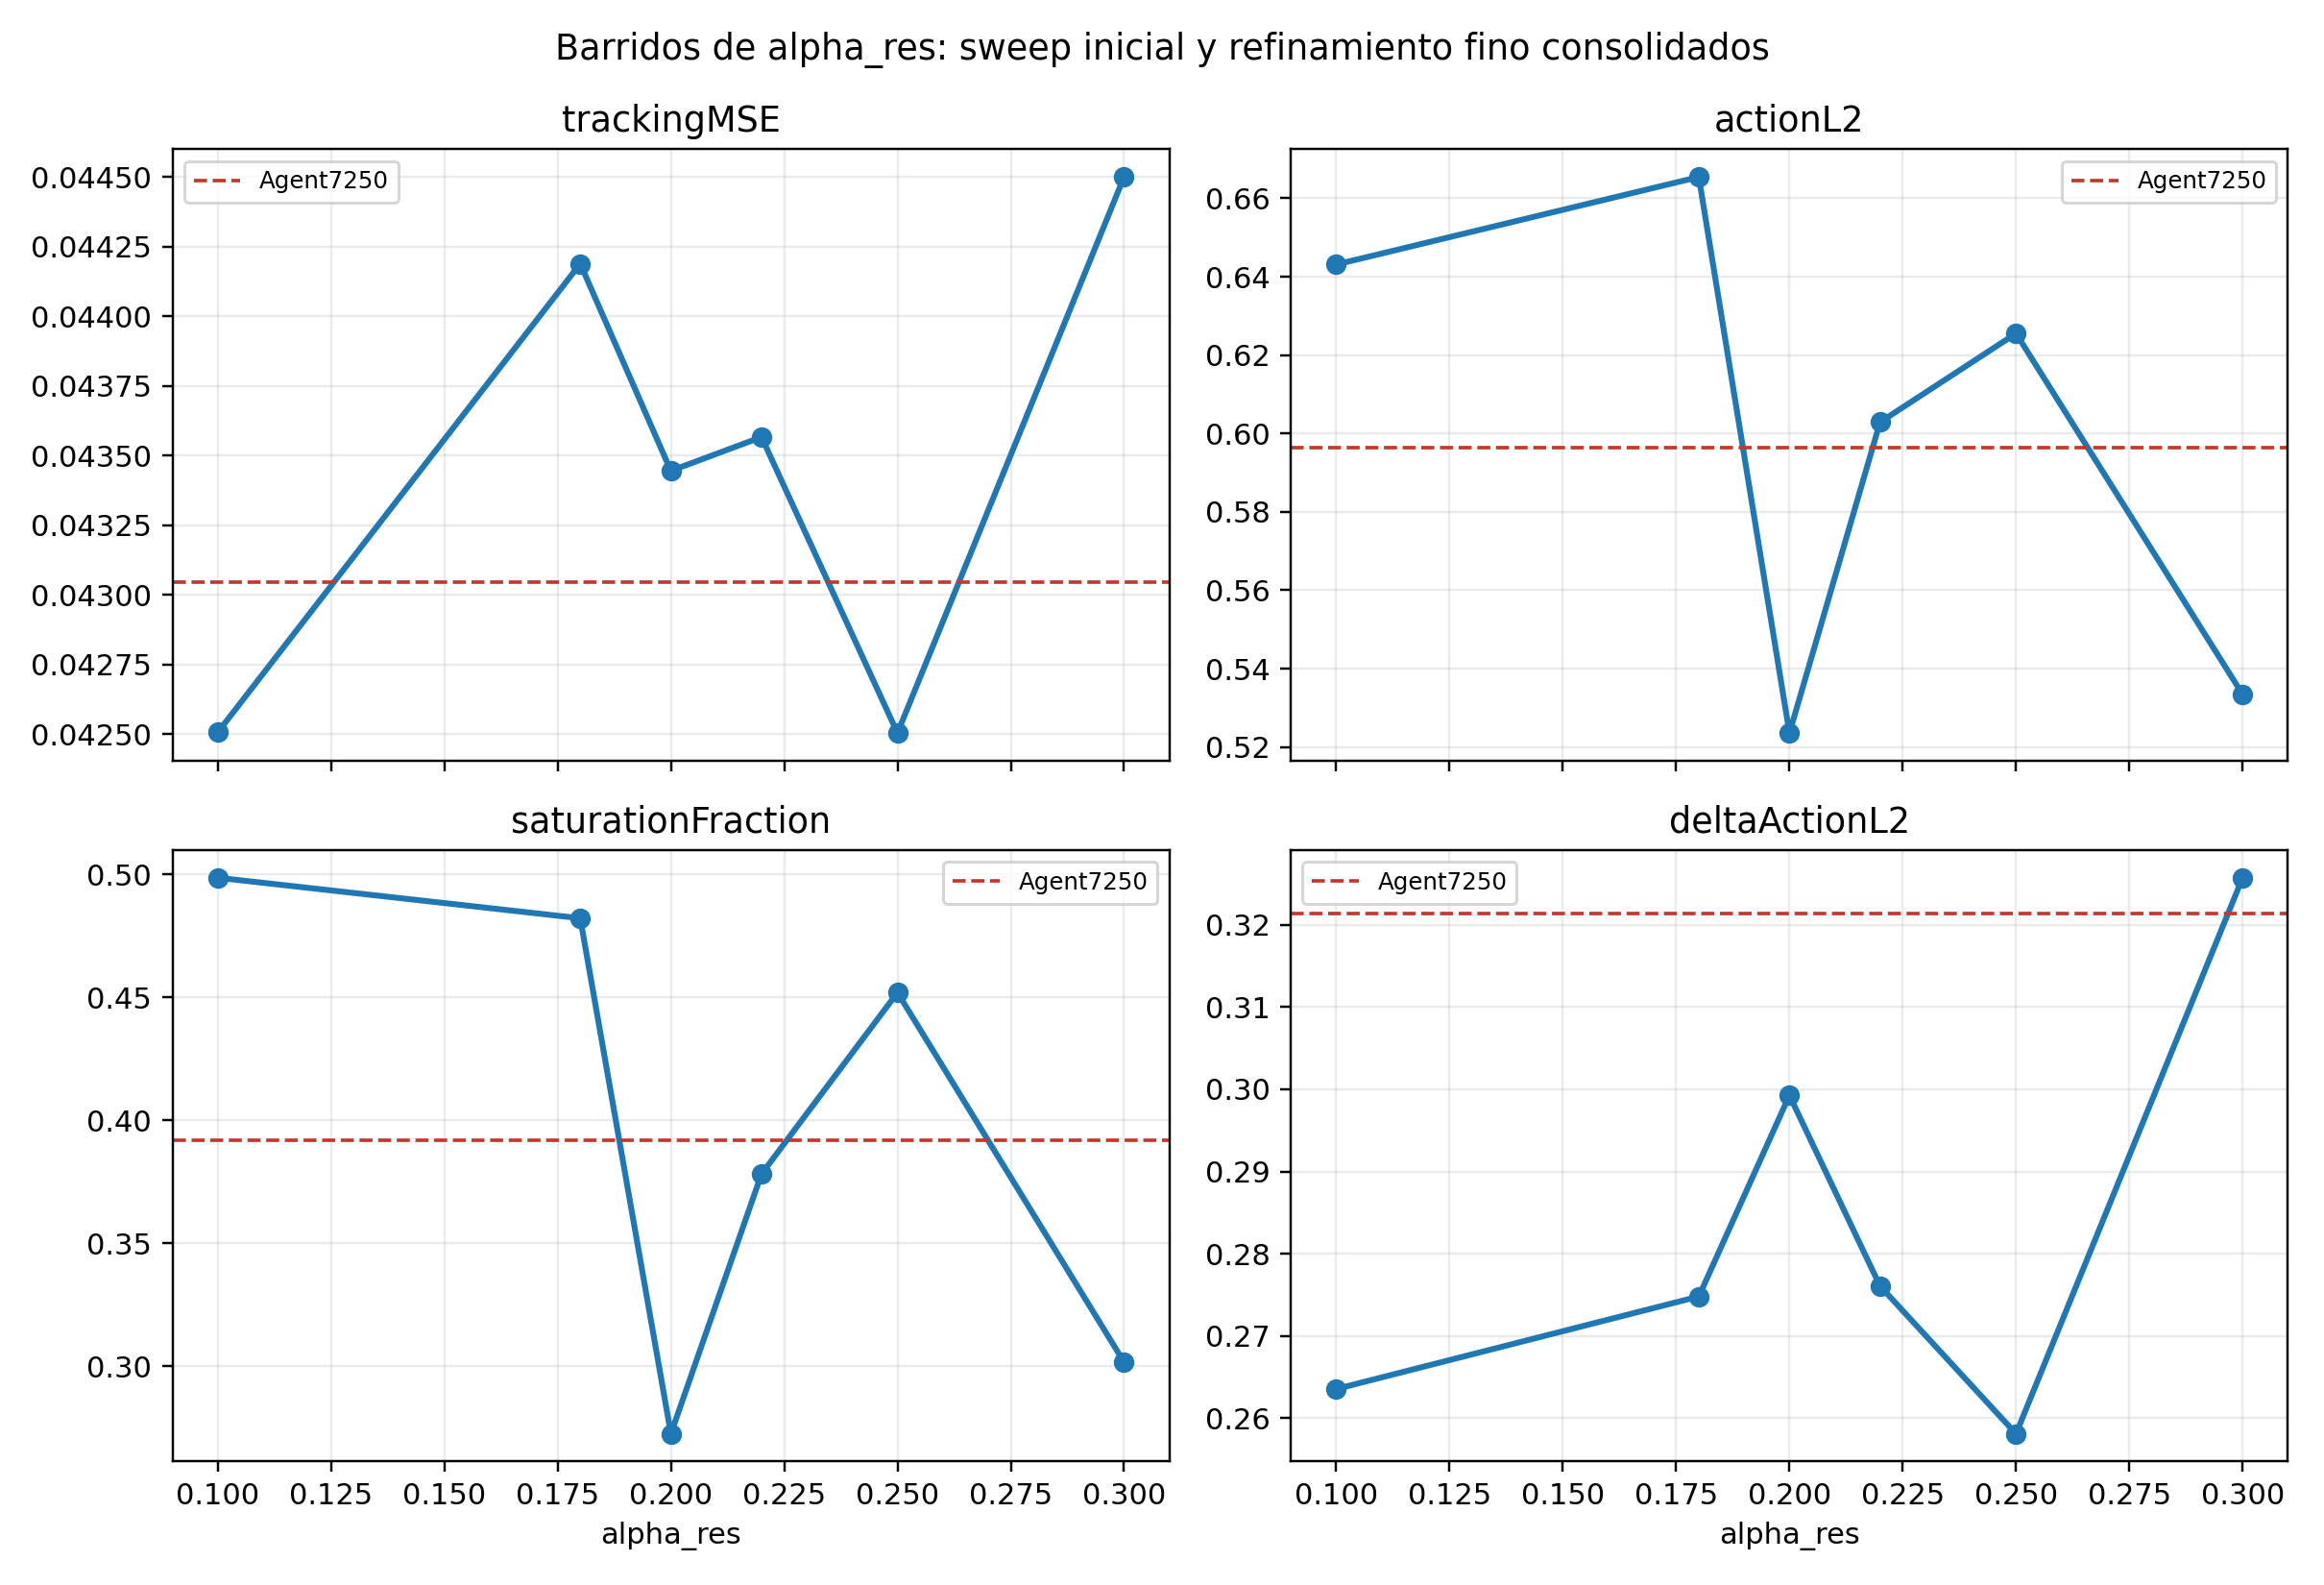
\includegraphics[width=0.97\linewidth]{figures/residual_alpha_sweep_metrics_20260326.png}
\caption{Metricas finales de los barridos de \(\alpha_{\mathrm{res}}\). Las lineas rojas discontinuas marcan el benchmark \texttt{Agent7250}.}
\end{figure}

\section{Resultados del refinamiento fino}

Una vez localizado \(0.20\) como zona fuerte, el refinamiento fino respondio si habia una mejora pequena y no obvia alrededor de ese valor.

\begin{table}[H]
\centering
\caption{Refinamiento fino de \(\alpha_{\mathrm{res}}\)}
\begin{tabular}{lrrrrl}
\toprule
\(\alpha_{\mathrm{res}}\) & trackingMSE & actionL2 & saturationFraction & deltaActionL2 & Estado final \\
\midrule
0.18 & 0.044189 & 0.665430 & 0.482118 & 0.274781 & Rejected \\
0.20 & 0.043445 & 0.523597 & 0.272637 & 0.299262 & ConditionB \\
0.22 & 0.043566 & 0.602889 & 0.378192 & 0.276052 & Rejected \\
0.25 & 0.042503 & 0.625515 & 0.451917 & 0.258078 & Rejected \\
\bottomrule
\end{tabular}
\end{table}

El refinamiento cerro la linea con bastante claridad:

\begin{itemize}[leftmargin=1.6em]
\item \(\alpha = 0.18\) no fue una version ``mas segura''; al contrario, salio peor en esfuerzo y saturacion.
\item \(\alpha = 0.22\) quedo cerca en tracking, pero ya perdia demasiada eficiencia en control.
\item \(\alpha = 0.25\) compro tracking a costa de mas borde y mas accion.
\item \(\alpha = 0.20\) siguio siendo el unico punto que sostuvo el compromiso completo.
\end{itemize}

\begin{figure}[H]
\centering
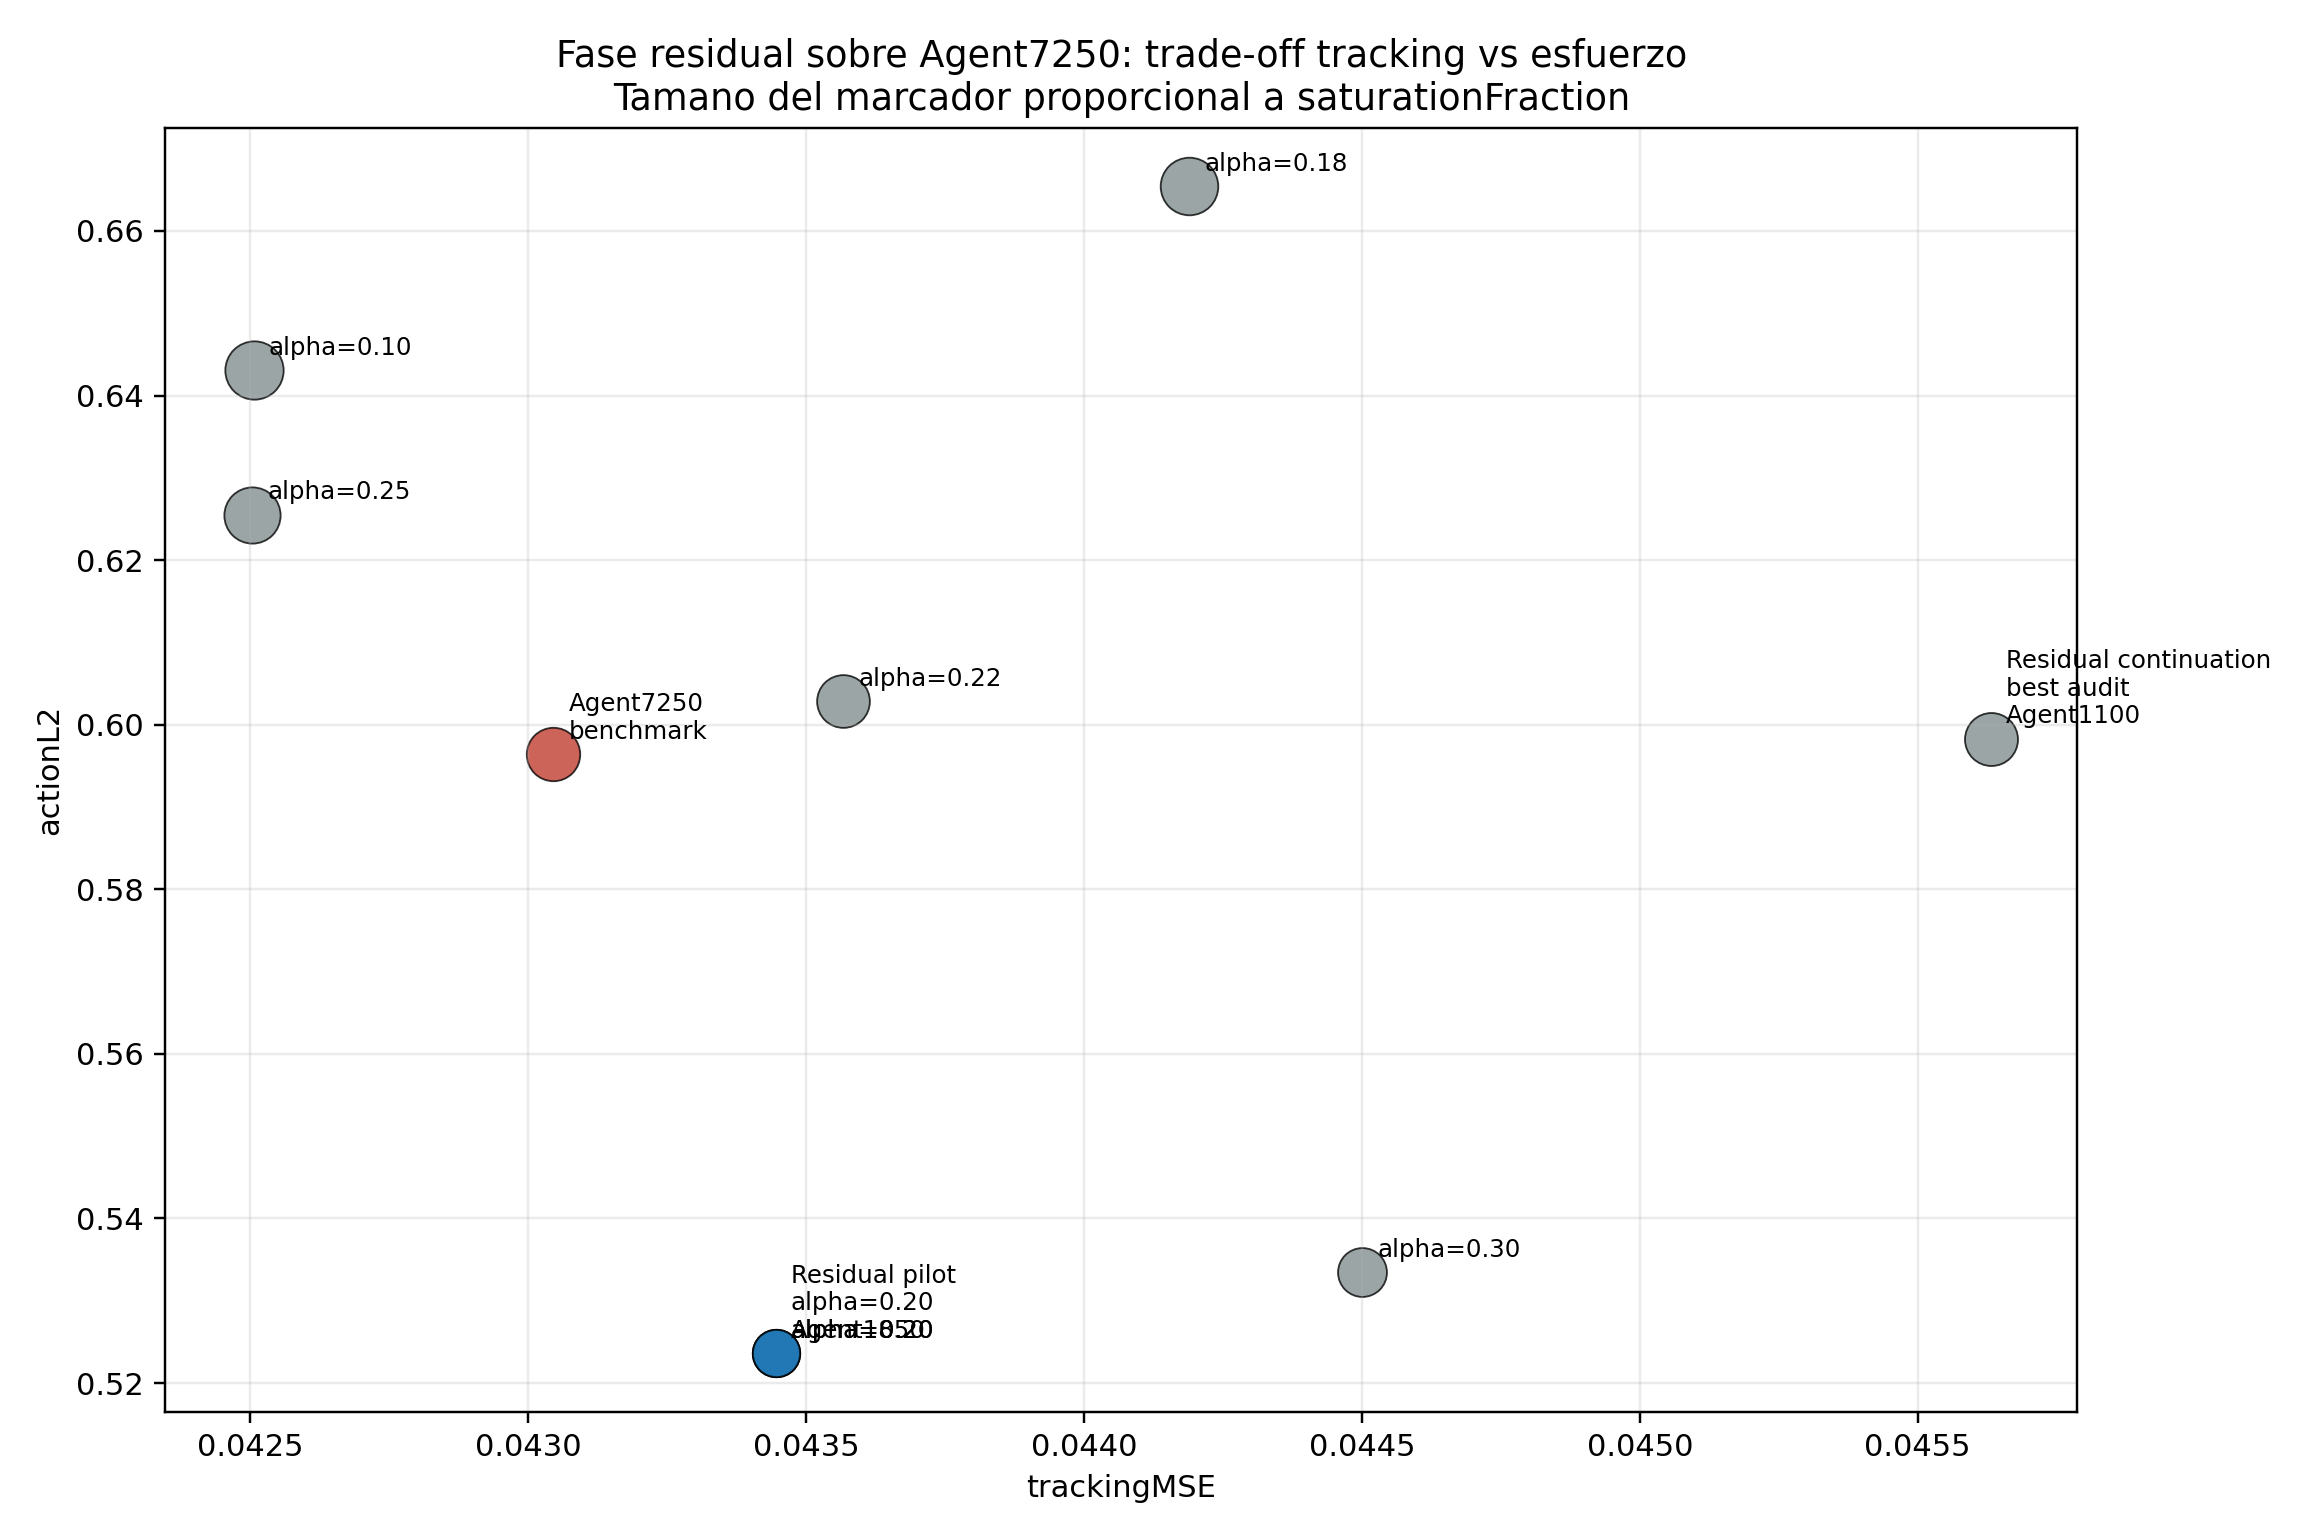
\includegraphics[width=0.98\linewidth]{figures/residual_phase_tradeoff_20260326.png}
\caption{Panorama completo de la fase residual. El tamano del marcador es proporcional a \texttt{saturationFraction}. El mejor candidato final sigue siendo el residual con \(\alpha=0.20\).}
\end{figure}

\section{Que dicen los diagnosticos residuales}

La ventaja de esta fase no fue solo encontrar un mejor agente; tambien permitio entender \emph{como} se aparta la politica residual respecto a la base.

Durante la auditoria se resumieron, entre otras, estas metricas:

\begin{itemize}[leftmargin=1.6em]
\item \texttt{auditResidualActionL2Mean}: magnitud media de la correccion residual.
\item \texttt{auditBaseToFinalActionDeltaMean}: cuanto se mueve la accion final respecto a la base.
\item \texttt{auditSignOverrideFractionMean}: con que frecuencia la residual cambia el signo de la accion base.
\end{itemize}

En el mejor caso, \(\alpha = 0.20\), esos valores fueron moderados:

\begin{itemize}[leftmargin=1.6em]
\item \texttt{ResidualActionL2Mean} \(\approx 0.0452\),
\item \texttt{BaseToFinalActionDeltaMean} \(\approx 0.0850\),
\item \texttt{SignOverrideFractionMean} \(\approx 0.0981\).
\end{itemize}

Eso es precisamente lo que se queria de una residual bien comportada: no colapsar a una politica totalmente distinta, sino corregir la base lo suficiente para rebajar agresividad sin perder casi todo el tracking.

\begin{figure}[H]
\centering
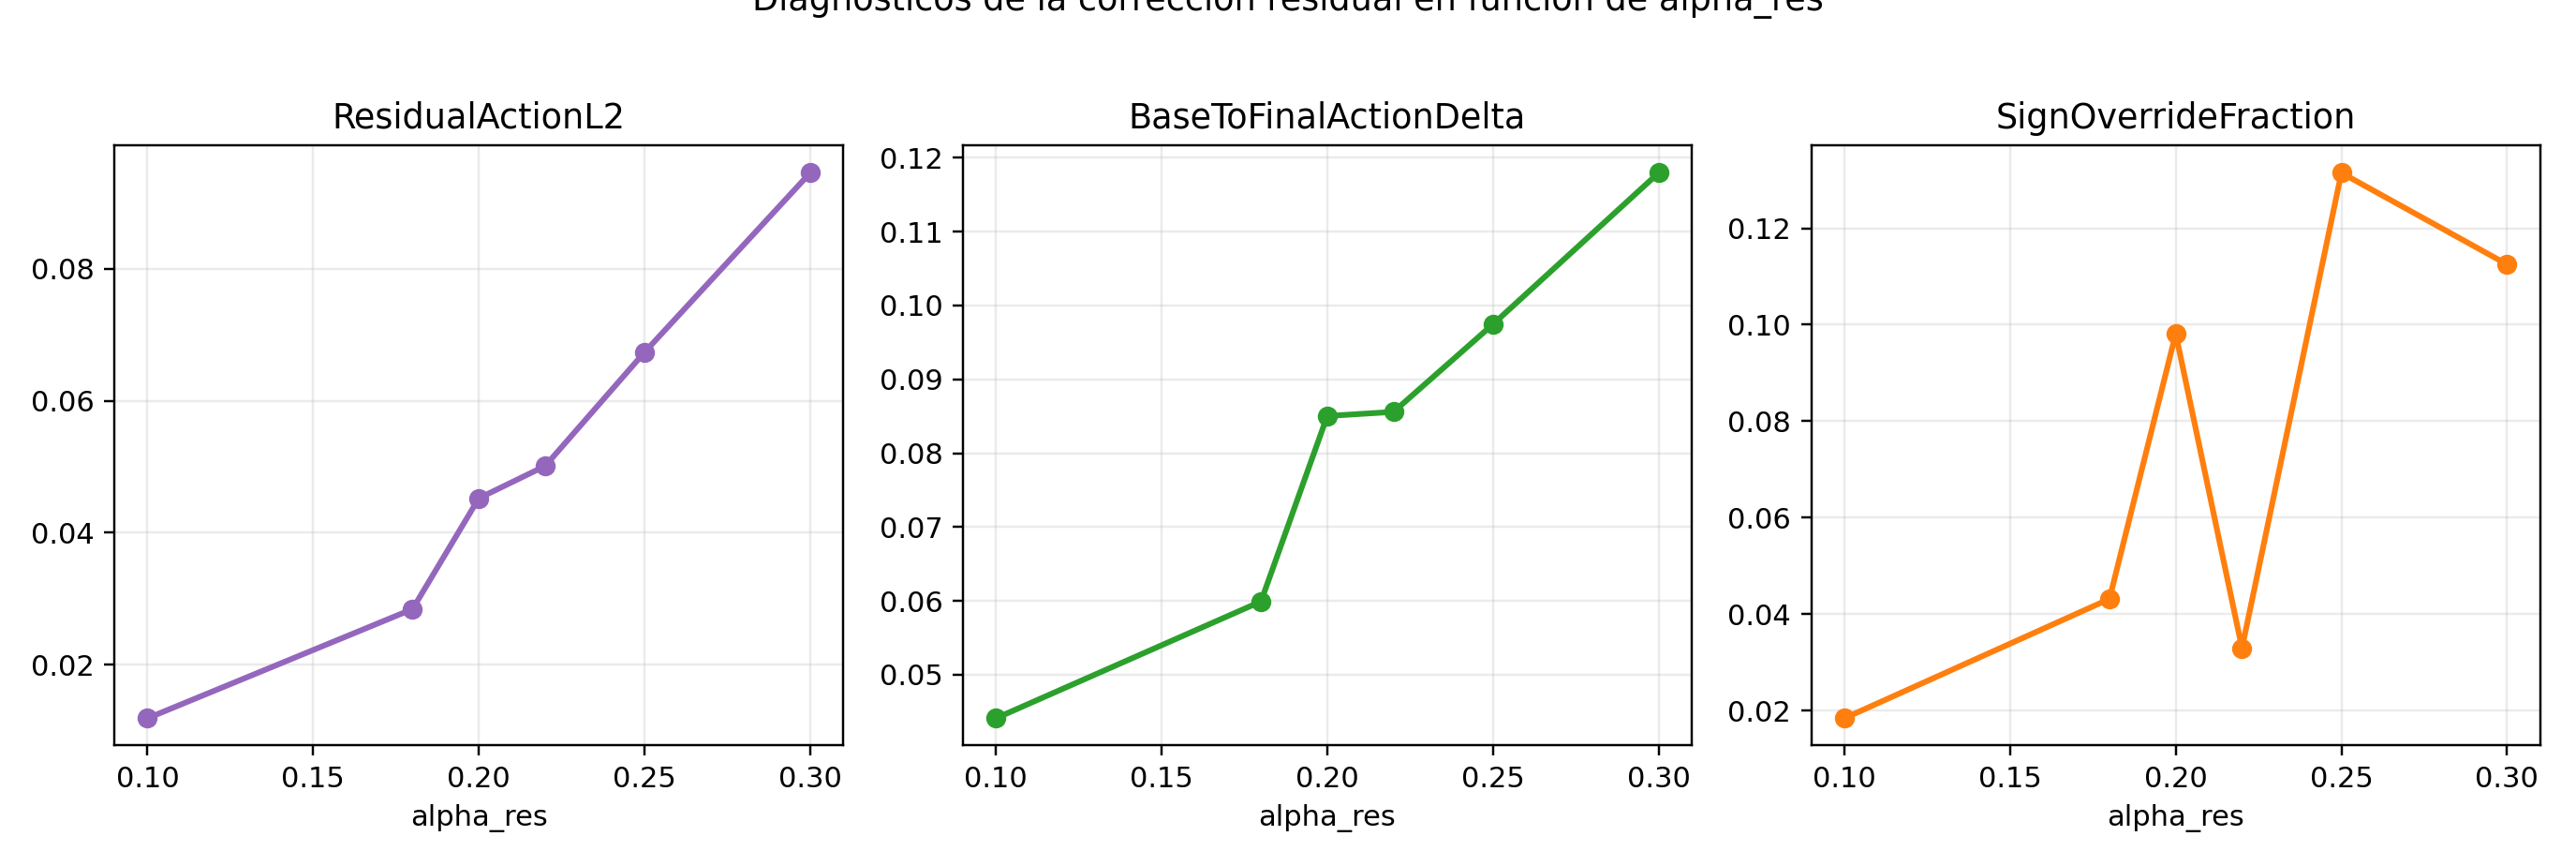
\includegraphics[width=0.98\linewidth]{figures/residual_alpha_diagnostics_20260326.png}
\caption{Diagnosticos de la correccion residual en funcion de \(\alpha_{\mathrm{res}}\). A mayor \(\alpha\), la residual gana capacidad para apartarse de la base; el punto util quedo en la zona intermedia.}
\end{figure}

\section{Interpretacion final de la fase}

La fase residual deja una conclusion mas fuerte que un simple ``este agente fue mejor'':

\begin{enumerate}[leftmargin=1.6em]
\item La idea residual estaba bien planteada. A diferencia de otras lineas recientes, si produjo una mejora real y defendible.
\item El mejor candidato actual del proyecto en esta familia es el residual \texttt{Agent1850} con \(\alpha_{\mathrm{res}} = 0.20\).
\item Entrenar mas, con la misma configuracion, no mejoro la politica.
\item Barrer \(\alpha\) tampoco encontro un punto mejor que \(0.20\), ni en el sweep corto ni en el refinamiento fino.
\item Por tanto, la linea residual no solo produjo una mejora: tambien quedo suficientemente localizada y cerrada desde el punto de vista metodologico.
\end{enumerate}

La leccion clave es que la mejora no vino de ``hacer otra reward'' ni de ``meter mas episodios'', sino de reorganizar la accion aprendida alrededor de una politica base fuerte. Ese es exactamente el tipo de escenario donde las ideas residuales son utiles \cite{silver2018residual,schaff2020shared,resfit2025}.

\section{Conclusion operativa}

Si el proyecto necesita fijar un candidato actual para entrega o documentacion final, la recomendacion tecnica ya es clara:

\begin{itemize}[leftmargin=1.6em]
\item benchmark historico congelado: \texttt{Agent7250},
\item mejor mejora encontrada sobre esa linea: residual \texttt{Agent1850} con \(\alpha_{\mathrm{res}} = 0.20\),
\item estado final frente al benchmark: \texttt{ConditionB}.
\end{itemize}

En otras palabras, la linea de trabajo que continuo realmente a \texttt{Agent7250} y aporto una mejora defendible fue la residual. Los barridos posteriores no la reemplazaron; la confirmaron.

\bibliographystyle{unsrt}
\bibliography{references}

\end{document}
